\documentclass[a4paper]{article}
\usepackage[a4paper,margin=0mm]{geometry}
\usepackage{fontspec}
\usepackage{unicode-math}
\usepackage{tikz}
\usepackage[table]{xcolor}
\usepackage[absolute]{textpos}
\usepackage{enumitem}
\usepackage{array}
\usepackage{multirow}

\setmainfont{Libertinus Serif}
\setsansfont{Libertinus Sans}
\setmathfont{Libertinus Math}
\newfontfamily\trackedsans{Libertinus Sans}[LetterSpace=8.0]

\definecolor{accent}{HTML}{602785}
\definecolor{badge}{HTML}{B8A0C8}
\definecolor{ink}{HTML}{2A2E30}

\setlength{\TPHorizModule}{1mm}
\setlength{\TPVertModule}{1mm}
\setlength{\parindent}{0pt}
\pagestyle{empty}

\newcommand{\LCOL}{16mm}
\newcommand{\RCOL}{111mm}
\newcommand{\COLW}{83mm}

\newcommand{\topicheader}[2]{%
\begin{textblock*}{194mm}(16mm,10mm)
\begin{tikzpicture}
\node[fill=accent,text=white,font=\sffamily\bfseries\fontsize{13}{13}\selectfont,
      minimum width=9mm,minimum height=9mm,inner sep=0pt] at (4.5mm,-4.5mm) {#1};
\node[font=\sffamily\bfseries\fontsize{15}{16}\selectfont,text=ink,anchor=west] at (12mm,-4.5mm) {#2};
\end{tikzpicture}
\end{textblock*}
\begin{textblock*}{194mm}(16mm,22.5mm)

\begin{tikzpicture}
\fill[accent] (0,0) rectangle (194mm,0.5mm);
\end{tikzpicture}
\end{textblock*}
}

\newcommand{\pagefooter}[1]{%
\begin{textblock*}{194mm}(8mm,286.41mm)
  
\begin{tikzpicture}
    \fill[accent] (0,0) rectangle (194mm,0.6mm);
  \end{tikzpicture}
\end{textblock*}
\begin{textblock*}{63.59mm}(8mm,288.27mm)
  {\sffamily\bfseries\color{accent}\fontsize{13}{16}\selectfont SAT 1200+}
\end{textblock*}
\begin{textblock*}{10mm}(188mm,288.27mm)
  \centering{\sffamily\color{accent}\fontsize{14}{16}\selectfont #1}
\end{textblock*}
}

\newcommand{\colrule}[2]{%
\begin{textblock*}{1mm}(105mm,#1mm)
\begin{tikzpicture}
\draw[black!65,line width=0.5pt] (0,0) -- (0,#2mm);
\end{tikzpicture}
\end{textblock*}
}

\newcommand{\setkicker}[2]{%
{\sffamily\bfseries\fontsize{12}{14}\selectfont #1.}\ {\itshape\fontsize{11}{14}\selectfont\color{black!75} #2}\par\vspace{2mm}%
}

\setlength{\fboxsep}{1.4pt}
\setlength{\fboxrule}{0.5pt}
\newcommand{\pnum}[1]{\fcolorbox{ink}{white}{\sffamily\bfseries\fontsize{8}{8}\selectfont #1}~}

\newcommand{\qrbox}[1]{%
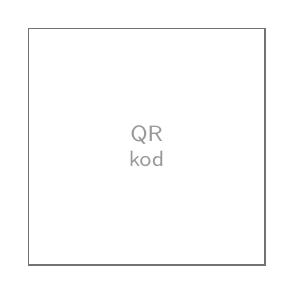
\begin{tikzpicture}
\draw[black!55,line width=0.6pt] (0,0) rectangle (30mm,30mm);
\node[black!40,font=\sffamily\fontsize{8}{9}\selectfont,align=center] at (15mm,15mm) {QR\\kod};
\end{tikzpicture}\\[1.5mm]
{\sffamily\fontsize{9}{11}\selectfont\color{black!70} #1}%
}

\arrayrulecolor{accent}
\setlength{\arrayrulewidth}{0.7pt}
\renewcommand{\arraystretch}{1.3}
\newcommand{\anstitle}[1]{{\sffamily\bfseries\color{accent}\fontsize{11}{13}\selectfont #1}\\[1.3mm]}

\begin{document}

% ================= PAGE 1: Set 1 | Set 2 =================
\topicheader{12}{Nochiziqli sistemalar}
\pagefooter{1}
\colrule{32}{238}
\mbox{}%

\begin{textblock*}{\COLW}(\LCOL,32mm)
{\fontsize{11.5}{14}\selectfont
\setkicker{1-to'plam}{Har bir sistemani yeching -- har biri ikkita $(x,y)$ juftlik beradi.}

\noindent\pnum{1} $y=x+1,\ \ y=x^2-1$\\[28mm]
\noindent\pnum{2} $y=2x,\ \ y=x^2-3$\\[28mm]
\noindent\pnum{3} $y=x-2,\ \ y=x^2-4$\\[28mm]
\noindent\pnum{4} $y=3x+2,\ \ y=x^2+2x$\\[28mm]
\noindent\pnum{5} $y=x+6,\ \ y=x^2$\\[28mm]
\noindent\pnum{6} $y=4x-3,\ \ y=x^2$
}
\end{textblock*}

\begin{textblock*}{\COLW}(\RCOL,32mm)
{\fontsize{11.5}{14}\selectfont
\setkicker{2-to'plam}{Chiziqli-kvadratik, qiyinroq koeffitsiyentlar bilan.}

\noindent\pnum{1} $y=2x-5,\ \ y=x^2-3x+1$\\[28mm]
\noindent\pnum{2} $y=2x+4,\ \ y=x^2+x-2$\\[28mm]
\noindent\pnum{3} $y=-3x+11,\ \ y=x^2-x+3$\\[28mm]
\noindent\pnum{4} $y=7,\ \ y=x^2-2$\\[28mm]
\noindent\pnum{5} $y=-x+2,\ \ y=x^2-5x+2$
}
\end{textblock*}

\clearpage

% ================= PAGE 2: Set 3 | Set 4 =================
\topicheader{12}{Nochiziqli sistemalar}
\pagefooter{2}
\colrule{32}{238}
\mbox{}%

\begin{textblock*}{\COLW}(\LCOL,32mm)
{\fontsize{11.5}{14}\selectfont
\setkicker{3-to'plam}{Natijaviy tenglamaning diskriminantini toping va nechta haqiqiy yechim borligini ayting.}

\noindent\pnum{1} $y=x,\ \ y=x^2+5$\\[24mm]
\noindent\pnum{2} $y=2x-1,\ \ y=x^2+4$\\[24mm]
\noindent\pnum{3} $y=-x,\ \ y=x^2+3$\\[24mm]
\noindent\pnum{4} $y=3x-2,\ \ y=x^2+2x+5$
}
\end{textblock*}

\begin{textblock*}{\COLW}(\RCOL,32mm)
{\fontsize{11.5}{14}\selectfont
\setkicker{4-to'plam}{Har ikkala tenglamaning bosh koeffitsiyenti bir xil -- $x^2$ ni yo'qotish uchun ayiring.}

\noindent\pnum{1} $y=x^2+3x+2,\ \ y=x^2-x+10$\\[24mm]
\noindent\pnum{2} $y=x^2+5x-1,\ \ y=x^2+x+7$\\[24mm]
\noindent\pnum{3} $y=x^2-2x+4,\ \ y=x^2+4x-8$\\[24mm]
\noindent\pnum{4} $y=2x^2+x-3,\ \ y=2x^2-3x+5$\\[24mm]
\noindent\pnum{5} $y=x^2+6x+1,\ \ y=x^2-2x+9$
}
\end{textblock*}

\clearpage

% ================= PAGE 3: Set 5 | Set 6 (spot the error) =================
\topicheader{12}{Nochiziqli sistemalar}
\pagefooter{3}
\colrule{32}{238}
\mbox{}%

\begin{textblock*}{\COLW}(\LCOL,32mm)
{\fontsize{10.5}{13}\selectfont
\setkicker{5-to'plam}{Sistemani yeching, lekin faqat so'ralgan miqdorni bering -- xom juftliklarni emas.}

\noindent\pnum{1} $y=x+1,\ y=x^2-1$ -- barcha yechimlarning \textbf{$y$-koordinatalari yig'indisini} toping.\\[14mm]
\noindent\pnum{2} $y=2x,\ y=x^2-3$ -- barcha yechimlarning \textbf{$x$-koordinatalari ko'paytmasini} toping.\\[14mm]
\noindent\pnum{3} $y=2x-5,\ y=x^2-3x+1$ -- ikkala yechim bo'yicha $x_1+x_2+y_1+y_2$ ni toping.\\[14mm]
\noindent\pnum{4} $y=4x-3,\ y=x^2$ -- ikkita $y$-qiymat orasidagi \textbf{musbat farqni} toping.\\[14mm]
\noindent\pnum{5} $y=x+2,\ y=x^2$ -- \textbf{kattaroq} $x$-qiymatli yechim uchun $x+y$ ni toping.
}
\end{textblock*}

\begin{textblock*}{\COLW}(\RCOL,32mm)
{\fontsize{10.5}{13}\selectfont
\setkicker{6-to'plam}{Xatoni toping -- buzilgan qadamni ayting, to'g'ri javobni bering.}

\noindent\pnum{1} $y=x+1,\ y=x^2-1$ ifodasida ko'rsatilgan yechimda xato bor:\\[1mm]
\hspace*{7mm}\textit{``$x^2-x-2=0 \Rightarrow (x-2)(x+1)=0 \Rightarrow x=2 \Rightarrow y=3$. Javob: $(2,3)$.''}\\[2mm]
\hspace*{7mm}Xato va to'g'ri javob: \makebox[52mm]{\dotfill}\\[8mm]

\noindent\pnum{2} $y=2x,\ y=x^2-3$ ifodasida ko'rsatilgan yechimda xato bor:\\[1mm]
\hspace*{7mm}\textit{``$x^2-2x-3=0 \Rightarrow x=3$ yoki $x=-1$. Javob: $x=3$, $x=-1$.''}\\[2mm]
\hspace*{7mm}Xato va to'g'ri javob: \makebox[52mm]{\dotfill}\\[8mm]

\noindent\pnum{3} $y=x^2+3x+2,\ y=x^2-x+10$ ifodasida ko'rsatilgan yechimda xato bor:\\[1mm]
\hspace*{7mm}\textit{``$x^2$ hadlarini olib tashlab: $(3x+2)+(-x+10)=0 \Rightarrow 2x+12=0 \Rightarrow x=-6$.''}\\[2mm]
\hspace*{7mm}Xato va to'g'ri javob: \makebox[52mm]{\dotfill}\\[8mm]

\noindent\pnum{4} $y=x,\ y=x^2+5$ ifodasida ko'rsatilgan yechimda xato bor:\\[1mm]
\hspace*{7mm}\textit{``$x^2-x+5=0$: $D=1-20=-19$. $D$ manfiy bo'lsa ham, $x=\frac{1\pm\sqrt{19}}{2}$ -- ikkita yechim topamiz.''}\\[2mm]
\hspace*{7mm}Xato va to'g'ri javob: \makebox[52mm]{\dotfill}
}
\end{textblock*}

\clearpage

% ================= PAGE 4: Set 7 (bonus) =================
\topicheader{12}{Nochiziqli sistemalar}
\pagefooter{4}
\colrule{32}{238}
\mbox{}%

\begin{textblock*}{\COLW}(\LCOL,32mm)
{\fontsize{11}{14}\selectfont
\setkicker{7-to'plam}{Bonus / qiyin -- har biriga taxminan 90 soniya.}

\noindent\pnum{1} $y=x^2-4x+1,\ \ y=x^2+2x-11$\\[28mm]
\noindent\pnum{2} $y=\dfrac{1}{2}x+1,\ \ y=x^2-x$\\[28mm]
\noindent\pnum{3} $y=2x+7,\ y=x^2+4x+10$ -- chiziq parabola bilan nechta kesishish nuqtasiga ega?\\[22mm]
\noindent\pnum{4} $y=4x-4,\ y=x^2$ -- urinish nuqtasini toping.
}
\end{textblock*}

\begin{textblock*}{\COLW}(\RCOL,32mm)
{\fontsize{11}{14}\selectfont

\noindent\pnum{5} $y=-2x+5,\ y=x^2-3x-1$ -- ikkita $y$-qiymat orasidagi \textbf{musbat farqni} toping.
}
\end{textblock*}

\clearpage

% ================= PAGE 5: Javoblar =================
\topicheader{12}{Nochiziqli sistemalar}
\pagefooter{5}
\mbox{}%

\begin{textblock*}{194mm}(16mm,28mm)
{\bfseries\itshape\color{accent}\fontsize{19}{21}\selectfont\centering Javoblar\par}
\end{textblock*}

\begin{textblock*}{194mm}(16mm,40mm)
{\fontsize{9}{11}\selectfont
\centering
\renewcommand{\arraystretch}{1.25}
\begin{tabular}{|>{\centering\arraybackslash}p{24mm}|>{\centering\arraybackslash}p{9mm}|>{\centering\arraybackslash}p{34mm}|>{\centering\arraybackslash}p{9mm}|>{\centering\arraybackslash}p{34mm}|}
\hline
\rowcolor{badge!55}\textbf{To'plam} & \textbf{\#} & \textbf{Javob} & \textbf{\#} & \textbf{Javob}\\
\hline
\multirow{3}{24mm}{\centering 1-to'plam} & 1 & $(2,3),(-1,0)$ & 2 & $(3,6),(-1,-2)$\\\cline{2-5}
 & 3 & $(2,0),(-1,-3)$ & 4 & $(2,8),(-1,-1)$\\\cline{2-5}
 & 5 & $(3,9),(-2,4)$ & 6 & $(1,1),(3,9)$\\\hline
\multirow{3}{24mm}{\centering 2-to'plam} & 1 & $(2,-1),(3,1)$ & 2 & $(3,10),(-2,0)$\\\cline{2-5}
 & 3 & $(2,5),(-4,23)$ & 4 & $(3,7),(-3,7)$\\\cline{2-5}
 & 5 & $(0,2),(4,-2)$ & -- & --\\\hline
\multirow{4}{24mm}{\centering 3-to'plam} & \multicolumn{4}{p{86mm}|}{1.\ $D=-19$, haqiqiy yechim yo'q}\\\cline{2-5}
 & \multicolumn{4}{p{86mm}|}{2.\ $D=-16$, haqiqiy yechim yo'q}\\\cline{2-5}
 & \multicolumn{4}{p{86mm}|}{3.\ $D=-11$, haqiqiy yechim yo'q}\\\cline{2-5}
 & \multicolumn{4}{p{86mm}|}{4.\ $D=-27$, haqiqiy yechim yo'q}\\\hline
\multirow{3}{24mm}{\centering 4-to'plam} & 1 & $(2,12)$ & 2 & $(2,13)$\\\cline{2-5}
 & 3 & $(2,4)$ & 4 & $(2,7)$\\\cline{2-5}
 & 5 & $(1,8)$ & -- & --\\\hline
\multirow{3}{24mm}{\centering 5-to'plam} & 1 & $3$ & 2 & $-3$\\\cline{2-5}
 & 3 & $5$ & 4 & $8$\\\cline{2-5}
 & 5 & $6$ \scriptsize{(nuqta $(2,4)$)} & -- & --\\\hline
\multirow{4}{24mm}{\centering 6-to'plam} & \multicolumn{4}{p{86mm}|}{1.\ Ikkinchi yechim $x=-1$ (va mos $y=0$) tushib qolgan. To'g'ri: $(2,3)$ \textbf{va} $(-1,0)$.}\\\cline{2-5}
 & \multicolumn{4}{p{86mm}|}{2.\ $x$ topilgan, lekin $y$ ga qaytarib qo'yilmagan. To'g'ri: $(3,6)$ va $(-1,-2)$.}\\\cline{2-5}
 & \multicolumn{4}{p{86mm}|}{3.\ Ikki ifoda qo'shilgan, tenglashtirilmagan. To'g'ri qadam: $3x+2=-x+10$. To'g'ri: $x=2$, $y=12$.}\\\cline{2-5}
 & \multicolumn{4}{p{86mm}|}{4.\ Manfiy diskriminant haqiqiy yechim yo'qligini bildiradi; $\sqrt{19}$ yozish buni to'g'rilamaydi. To'g'ri: haqiqiy yechim yo'q.}\\\hline
\multirow{3}{24mm}{\centering 7-to'plam} & 1 & $(2,-3)$ & 2 & $(2,2),(-\frac12,\frac34)$\\\cline{2-5}
 & 3 & $D=-8$, $0$ ta & 4 & $(2,4)$ (qo'sh ildiz)\\\cline{2-5}
 & 5 & $10$ & -- & --\\\hline
\end{tabular}
}
\end{textblock*}

\begin{textblock*}{194mm}(16mm,245mm)
\centering
{\sffamily\fontsize{9.5}{11.5}\selectfont\color{black!70} Video yechimlar va qo'shimcha testlar uchun quyidagi QR kodlarni skanerlang:}\\[4mm]
\begin{minipage}[t]{32mm}\centering\qrbox{YouTube}\end{minipage}%
\hspace{16mm}%
\begin{minipage}[t]{32mm}\centering\qrbox{Telegram}\end{minipage}
\end{textblock*}

\end{document}
